In this exercise the task at hands is to clone one image into another, using seamless image cloning as can be seen in \cref{fig:cloning}. The given code for this exercise is very sparse, providing only the calls to a function \texttt{your\_blend} which is empty of functionality, but does contain some description of the work which has to be done.\\

To do this a few new concept is used such as double buffering, which uses two buffers, one which is used to perform computations on, from which the result is written into the second buffer. In the next iteration, the roles of the buffers are then swapped, and the same computations are done again. Other things include creating a mask from the source image to determine border and interior pixels on the polar bear image, and transposing RGB values, to separate into array of channel values instead of array of RGB values.\\

Last, to do the "merging" part of the cloning process solves a Poisson equation to determine how the image is to be blended. To solve the Poisson equation the exerciser gives a method, based on Jacobi Iterations, which provides the following formula for computing the value of a pixel:

\begin{align*}
I_{k+1} &= \frac{A + B + C}{D}
\end{align*} 

To determine A, B, C and D the concept neighbors is used, which is the index of the pixels besides the given pixel. Neighbors can only be with on or within the border of the mask created. Using this, A, B, C, D is as follows:

\begin{itemize}
	\item A is sum of the pixels interior neighbors in the buffer
	\item B is the sum of the pixels border neighbors in the target image
	\item C is difference between the pixel and its neighbors on the source image
	\item D is number of neighbors.
\end{itemize}

This computation is done for each of the channels which in the image, thus for R, G and B., In the end, the three individual channels are combined to make a whole image.

\begin{figure}[ht]
	\centering
	\fbox{
		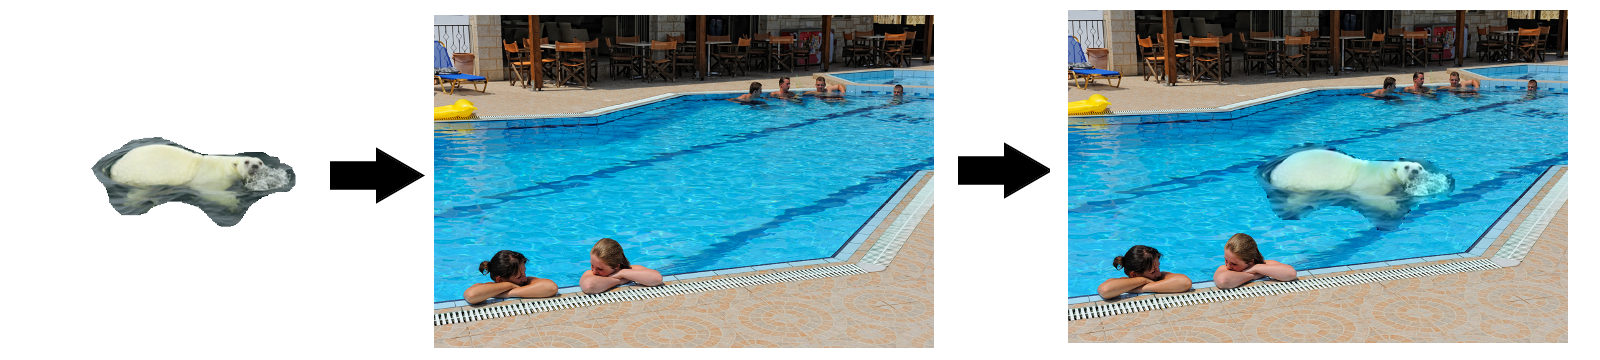
\includegraphics[width=0.9\textwidth]{figs/exercises/ex6/merged.png}
	}
	\caption{The source image of a polar bear is to be cloned onto a destination picture of an swimming pool.}
	\label{fig:cloning}
\end{figure}

There are several steps involved in implementing this task, here the task is divided into work, corresponding to the kernels, being called in the solution:
\begin{enumerate}
	\item[\textbf{Step 1}]
	The first step is to create the mask, based on the source image, to determine the border and interior pixels of the source image. The source image contains either some RGB value or else (255, 255, 255) for everything that is not supposed to be cloned into the destination. These values can then be used for creating the mask inside a kernel.
	\item[\textbf{Step 2}]
	Transpose both the source and destination image from RGB values to separate arrays for each color channel.
	\item[\textbf{Step 3}]
	Assign the initial value for the guess to solving the Poisson equation to each of the two buffers. The initial value used is the one from the source image.
	\item[\textbf{Step 4}]
	Run the Jacobi iterations 800 times as assign by the exercise. This will give an approximation that is converging towards the correct solution. The Jacobi kernel performs the before mentioned equation in each iteration, based on the input buffer, and assigns the values to the output buffer. After each iteration, the two buffers are swapped.
	\item[\textbf{Step 5}]
	Lastly after 800 iterations the output buffer for each color channel is used to construct a combined image, which is the completed result of the seamless image clone.


\end{enumerate}